\setchapterstyle{kao}
\pagelayout{margin}
\setchapterimage{chargers-title3}
\setchapterpreamble[u]{\margintoc}
\chapter{Data}
\label{ch:data}

\footnotetext{Title image is a map o f Prague with all chargers denoted as triangles in available datasets. The layer below displays all buildings in Prague with color being the number of floors}




In this chapter types data will be introduced, how they are classified and data formats in which they were obtained. Chargers, charging session dat and some lightweitght ontology will be described. Then followed with transformations of charging sessions into \acrlong{APC} which will be target variable in our model.

Then data that are considered and used to predict \acrlong{APC} will be introduced together with their transformation into a desirable form for our model.

Some of the data have not been used but are part of data landscape considered and hold usefull information on what was thought might have an effect but in fact did not have.


\begin{kaobox}[frametitle=Types of data]

    \begin{itemize}
        \item \textbf{spatial}(geospatial) data are those which have assigned position in real world and are invariant in some timeframe. Such data are locations of \acrlong{CS}, administrative boundaries, road network, buildings.
        \item \textbf{temporal} data are characterized by their variation over time without specific geographical coordinates. In this thesis, these include charging session durations, energy consumption patterns throughout the day, historical charger utilization rates, and seasonal variations in charging demand.
        \item \textbf{spatio-temporal} data incorporate both location and time elements, providing insights into how phenomena evolve across space and time. Examples relevant to this research include mobility patterns of people, real-time charger availability, and dynamic variations in \acrshort{APC} across different city zones during different hours of the day.
    \end{itemize}
\end{kaobox}

\section{EV Chargers and Charging Sessions}

\subsection{Description}

\begin{figure}
    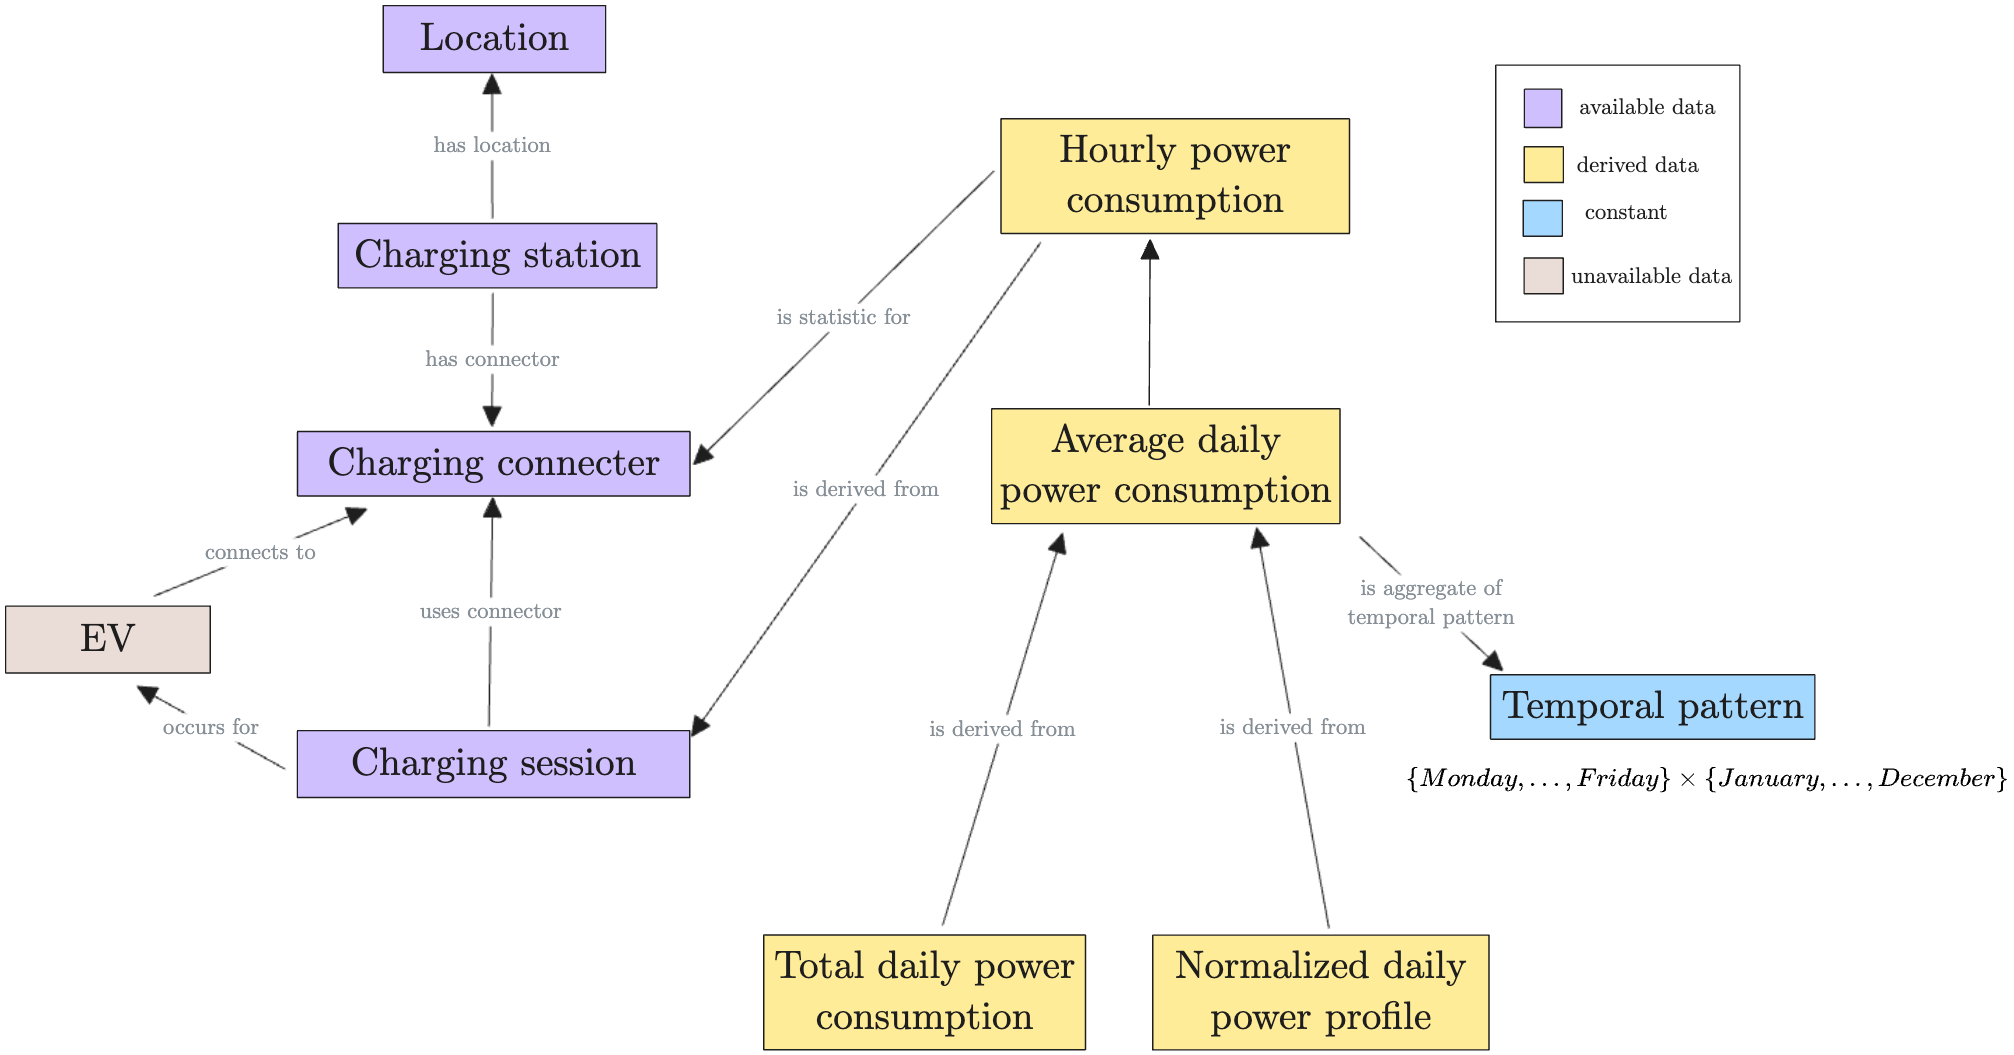
\includegraphics[width=1\textwidth]{data/charger-ontology.png}
    \caption{A charging ontology}
    \label{fig:charging-ontology}
\end{figure}


To introduce our problem domain and a possiblity to connect the data and how they relate. An simple charger ontology is introduced \sidenote{Ontology describe subjects of some system and a way how they are related together.}. Inspired by AURORAL EV-charger Ontology \sidecite{OntologyDocumentationGenerated} an ontolgoy of EV charging is introduced. The scope of it is to aide in understanding of the domain in this thesis.

The model matches data obtained from PRE.

Below is description of individual parts of the charging ontology as visible in \ref{fig:charging-ontology}.

\begin{itemize}
    \setlength\itemsep{1em}
    \item \textbf{\acrlong{CS}} (as visible in \ref{fig:charging-station}) is equipment that connects an \acrshort{EV} to a source of electricity to recharge them. A charging station typically consists of physical infrastructure including power conversion hardware, connectivity modules, authentication systems, and user interfaces. Charging stations vary in their power delivery capabilities, ranging from slow AC chargers (3.7-22 kW) commonly found in residential and workplace settings to fast DC chargers (50-350+ kW) deployed in public corridors and commercial hubs. Within our dataset, charging stations from PRE's network predominantly consist of public AC and DC installations distributed throughout Prague's urban and suburban areas.

          \begin{marginfigure}
              \centering
              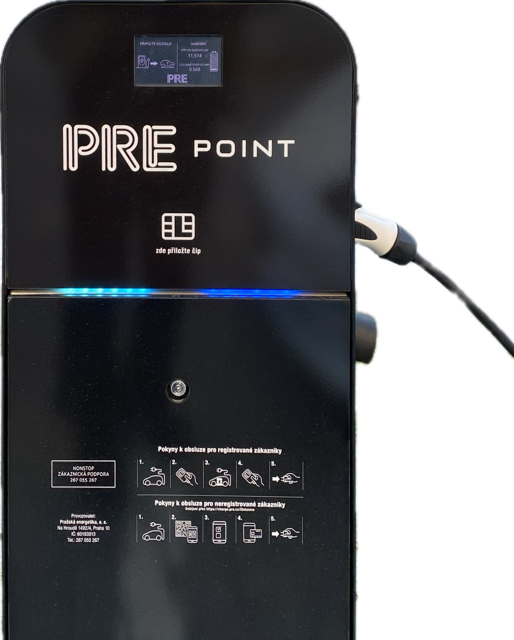
\includegraphics[width=0.42\textwidth]{data/charger-small.png}
              \caption{Picture of \acrlong{CS}. It has one connector on each of its sides. One of which has charging cable attached.}
              \label{fig:charging-station}
          \end{marginfigure}
          \vspace{3.5mm}
          Formally, we define the set of all charging stations as $S = \{s_1, s_2, ..., s_m\}$, where each station $s \in S$ is associated with a location $l_s \in \mathbb{R}^2$ representing its geographic coordinates.

    \item  \textbf{\acrlong{CP}} (as visible in \ref{fig:charging-connector}) one or many are part of a \acrshort{CS}. These physical interfaces allow for the actual connection between the vehicle and the charging inftrastructure. Connectors follow different standards depending on region and charging speeds. Each connector type supports specific charging protocols and power levels. In our studied network, the majority of charging stations feature multiple connectors (typically two to four), enabling simultaneous charging of different vehicles and supporting various connector standards to accommodate the heterogeneous EV market.

          \begin{marginfigure}
              \centering
              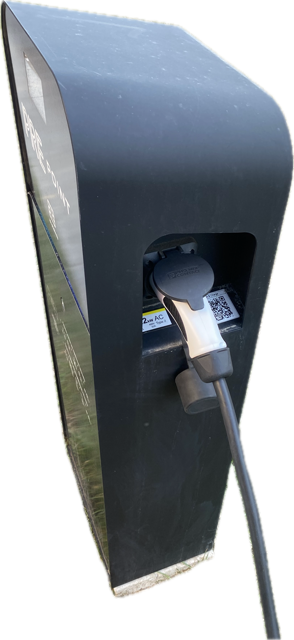
\includegraphics[width=0.3\textwidth]{data/charger-conector-small.png}
              \caption{View of 1 of the 2 charging connectors the \acrshort{CS} has}
              \label{fig:charging-connector}
          \end{marginfigure}
          \vspace{3.5mm}
          For each station $s \in S$, we define the set of connectors as $C_s = \{c_1^s, c_2^s, ..., c_{n_s}^s\}$, where $n_s$ represents the number of connectors at station $s$. Each connector $c \in C_s$ has a unique identifier $\text{id}^{c,s}$ assigned by PRE.

    \item \textbf{\acrlong{CSS}} occurs when an \acrshort{EV} arrives at a \acrshort{CS} and connects to a \acrshort{CP}. This interaction initiates a session that is logged by the \acrshort{CS} together with various parameters including connection time, disconnection time and total power consumed. The charging session captures both spatial, temporal patterns (duration, time of day, day of week) and energy consumption behaviors.

          \vspace{3.5mm}

          For each connector $c \in C_s$ at station $s$, we define the set of charging sessions as $V_{c,s} = \{v_1^{c,s}, v_2^{c,s}, ..., v_{k_{c,s}}^{c,s}\}$, where each session $v_i^{c,s} = (t_{\text{start},i}^{c,s}, t_{\text{end},i}^{c,s}, p_i^{c,s})$ is characterized by its start time, end time, and energy consumed during the session.

    \item \textbf{location} denotes the geographical position where the charger is installed. This spatial attribute is helpfull to our analysis framework as it allows for correlation between charging demand and various features of the surrounding environment.

          \vspace{3.5mm}

          The location function $l: S \rightarrow \mathbb{R}^2$ maps each station $s \in S$ to its geographic coordinates.

\end{itemize}

\subsubsection{Power consumption assumption}

\begin{marginfigure}
    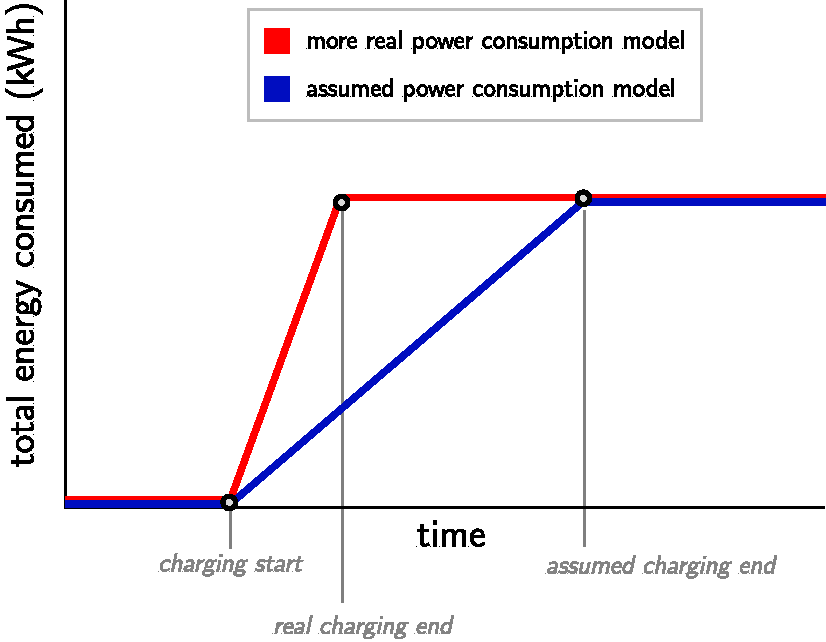
\includegraphics{charging-assumption.pdf}
    \caption[Charging assumption]{Chart comparing realistic power consumption vs our assumption.}
    \label{fig:charging-assumption}
\end{marginfigure}

Before we describe how \acrlong{CSS} have been processed into \acrlong{HPC} and \acrlong{APC}. In our model, we take simplyfing assumption on how actual power consumed during chargins session is consumed. Since actual power consumed can vary during charging of the electric vehicle. Most important is, the vehicle from connection time is being charged with the maximum power the \acrlong{EV} can handle and \acrlong{CP} can provide. This leads to charging session being split into two parts. First is charging part, that is when power is being delivered to the vehicle. And idle period where the vehicle has been fully charged and no power is being consumed\sidenote{Some charging station providers financially penalize this period of time, as an other \acrshort{EV} could have been charging. This can lead to improved availabilty of \acrlong{CS}.}. This is ilustrated in \ref{fig:charging-assumption}.

\subsection{Charging Sessions Dataset}

PRE provided us with charging session data collected from X charging stations across Prague. The dataset contains Y individual charging sessions. Spanning from January 2022 until June 2024  For each session, the following information is recorded:

\begin{itemize}
    \item \textbf{Charger ID}: A unique identifier assigned by PRE to each charger and connector
    \item \textbf{\acrlong{CS} location}: The physical address of the charging station
    \item \textbf{Connector type}: Categorized as AC, DC, or UFC
    \item \textbf{Session timestamps}: Start and end times of each charging session
    \item \textbf{Energy consumption}: Total power consumed during the session
\end{itemize}


The precise location of chargers has been identified with use of other supporting document from PRE.

\begin{figure}[]
    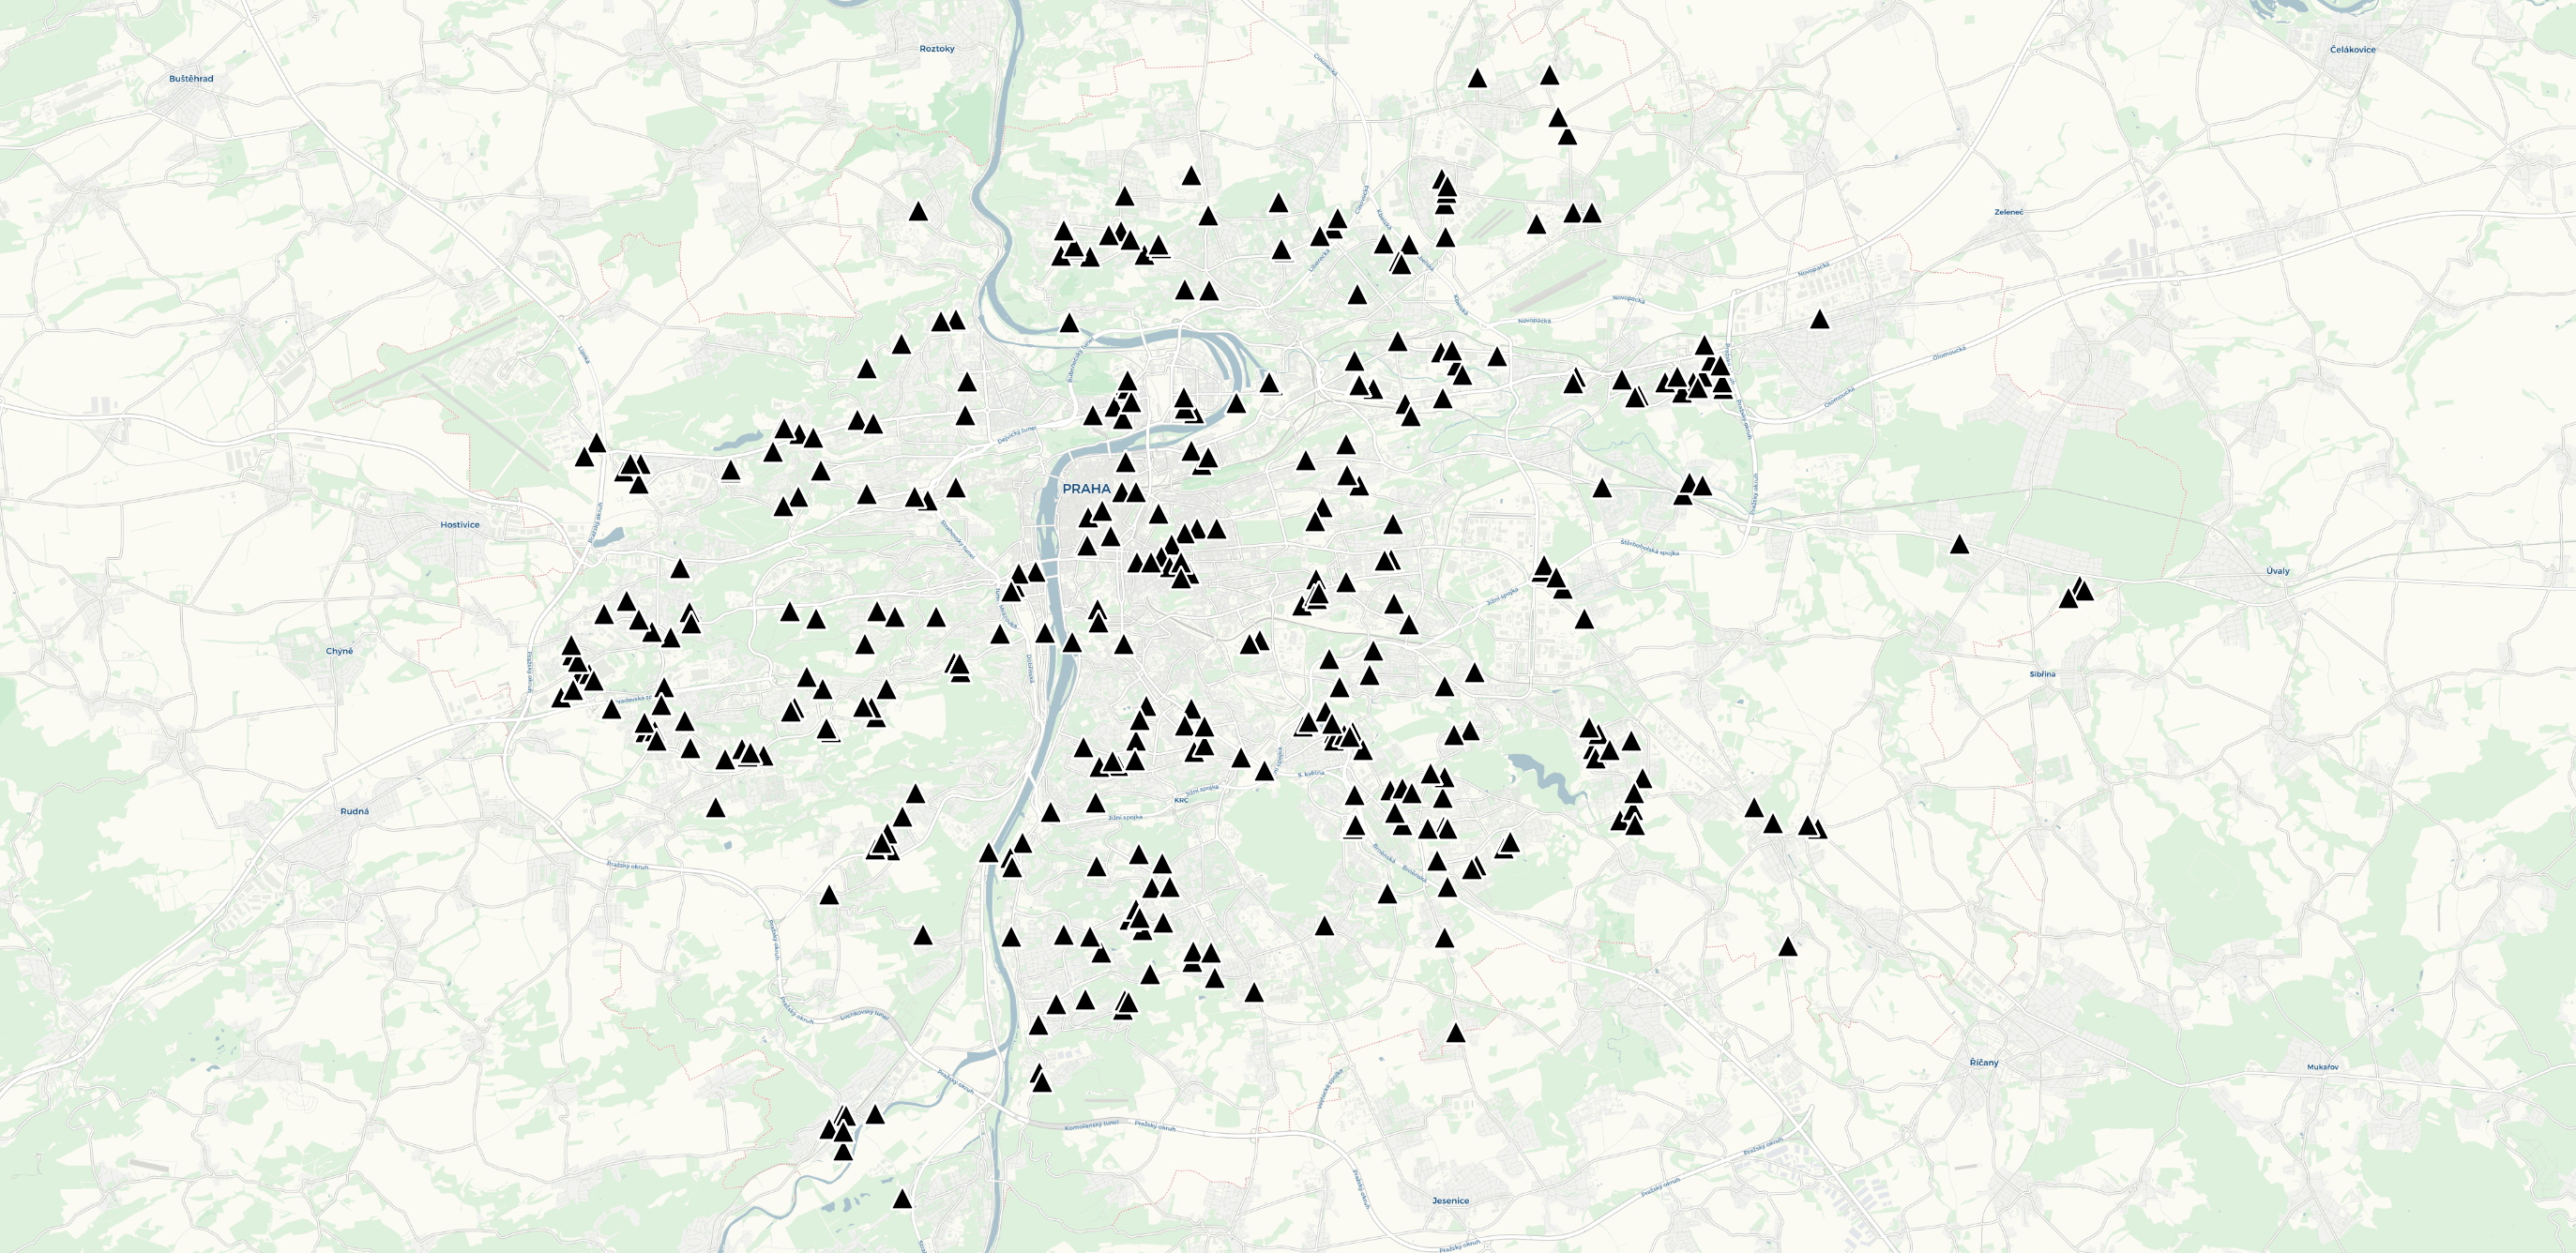
\includegraphics{data/all-chargers.png}
    \caption{}{Map of all PRE \acrlong{CS} in Prague for which we have available \acrlong{CSS}, See \ref{fig-large:all-chargers} for larger image.}
\end{figure}

\begin{marginfigure}
    \begin{tabular}{cc}
        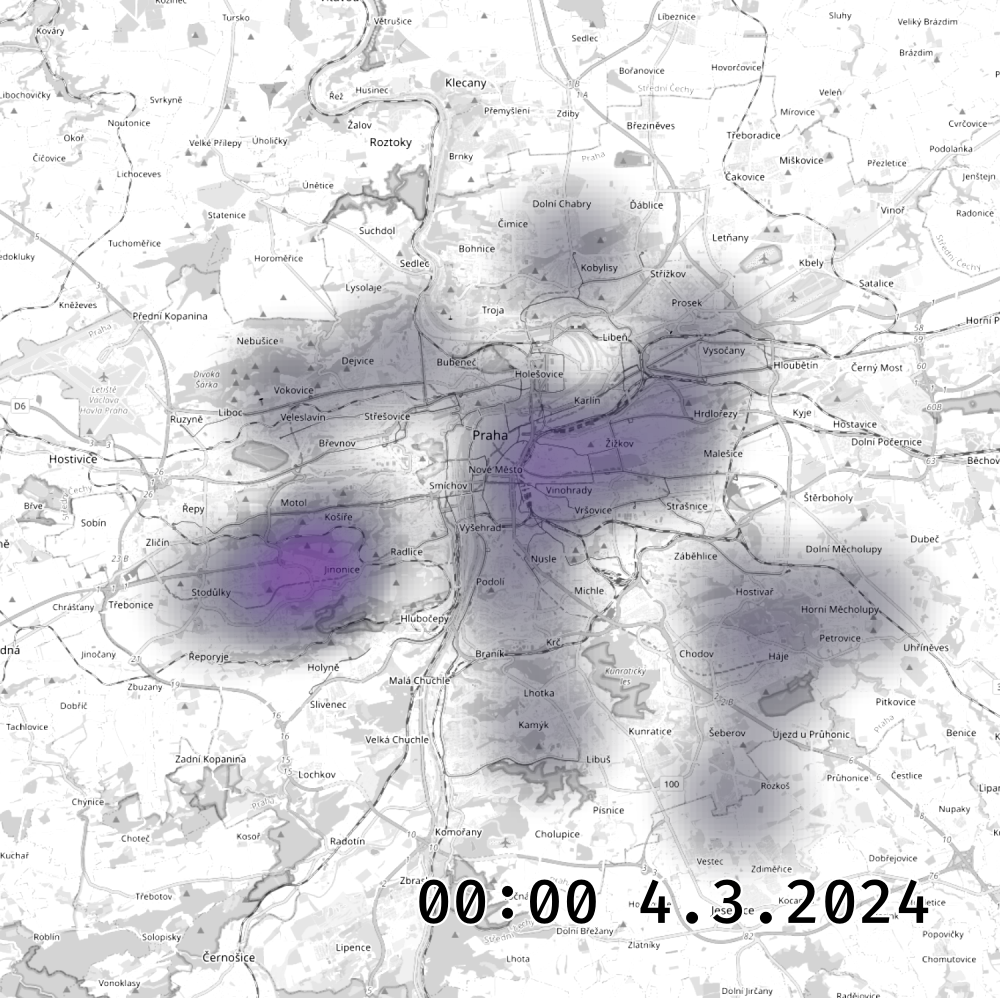
\includegraphics[width=0.45\marginparwidth]{data/timelapse/timelapse0000.png} &
        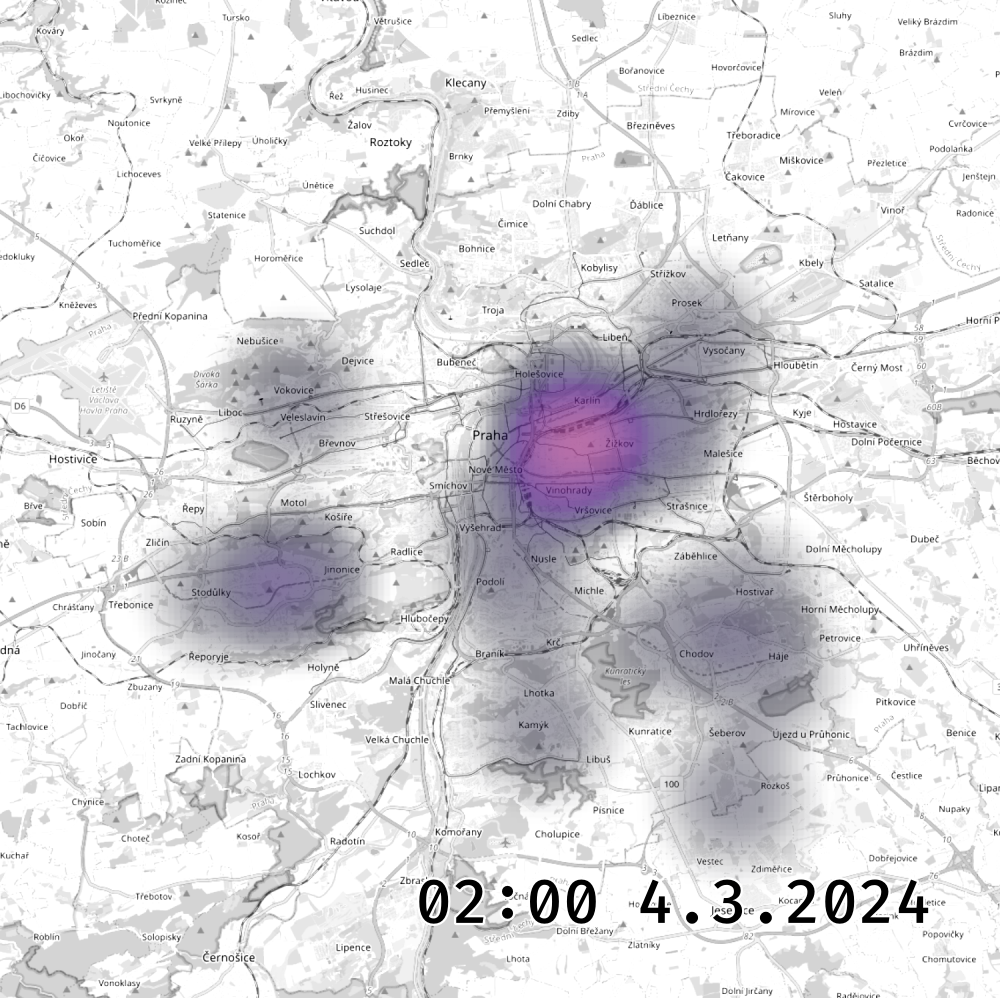
\includegraphics[width=0.45\marginparwidth]{data/timelapse/timelapse0001.png}   \\
        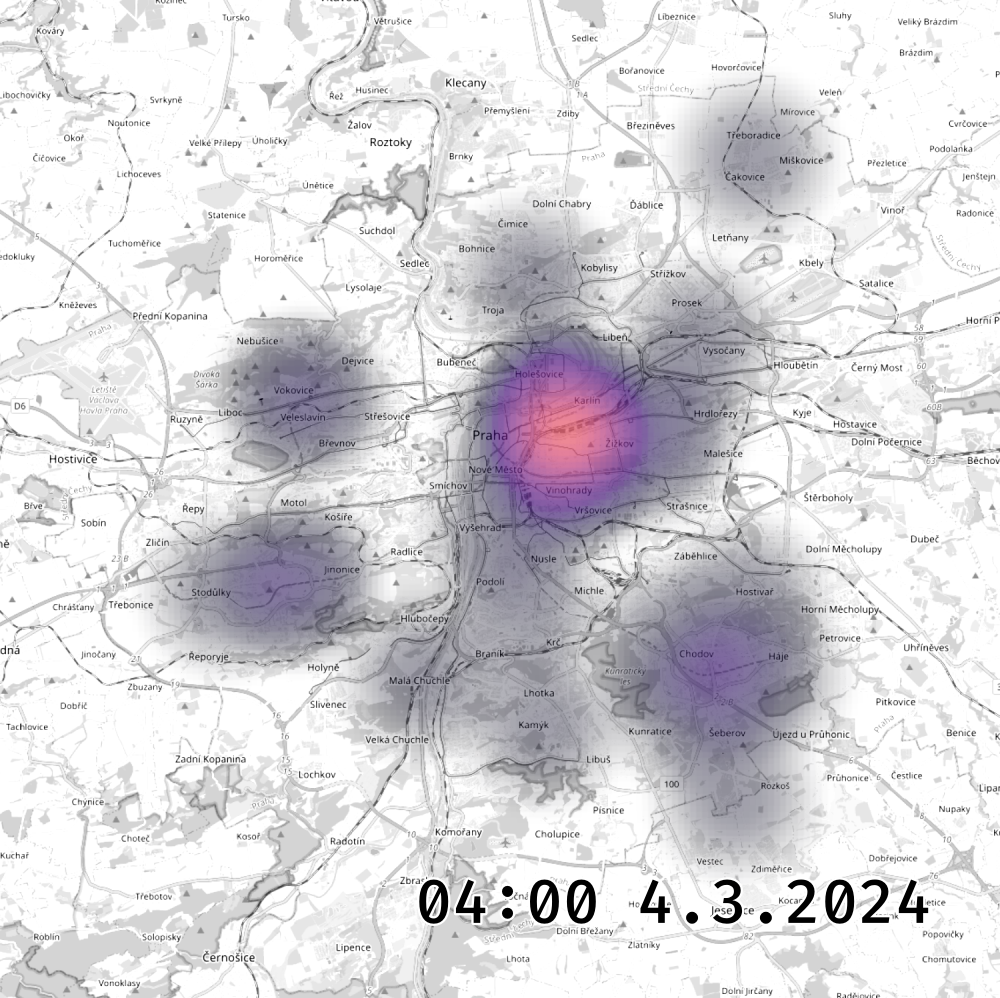
\includegraphics[width=0.45\marginparwidth]{data/timelapse/timelapse0002.png} &
        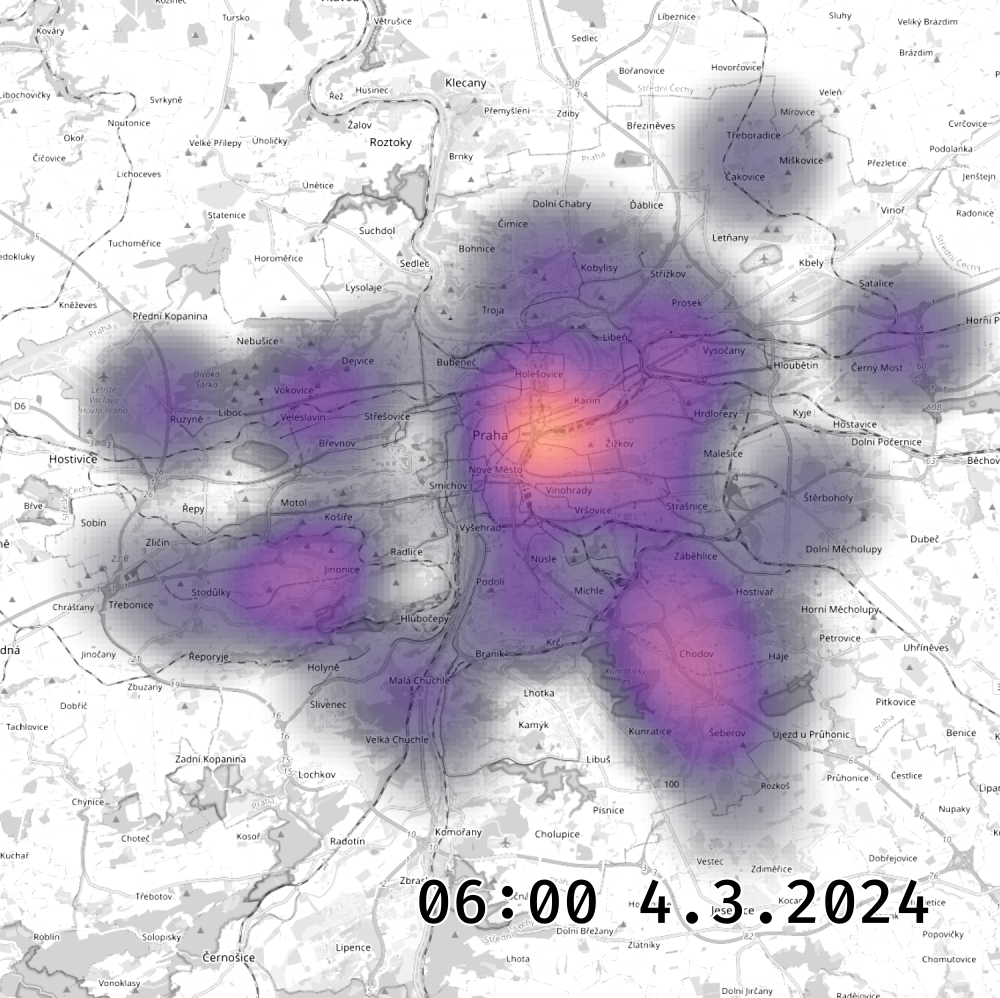
\includegraphics[width=0.45\marginparwidth]{data/timelapse/timelapse0003.png}   \\
        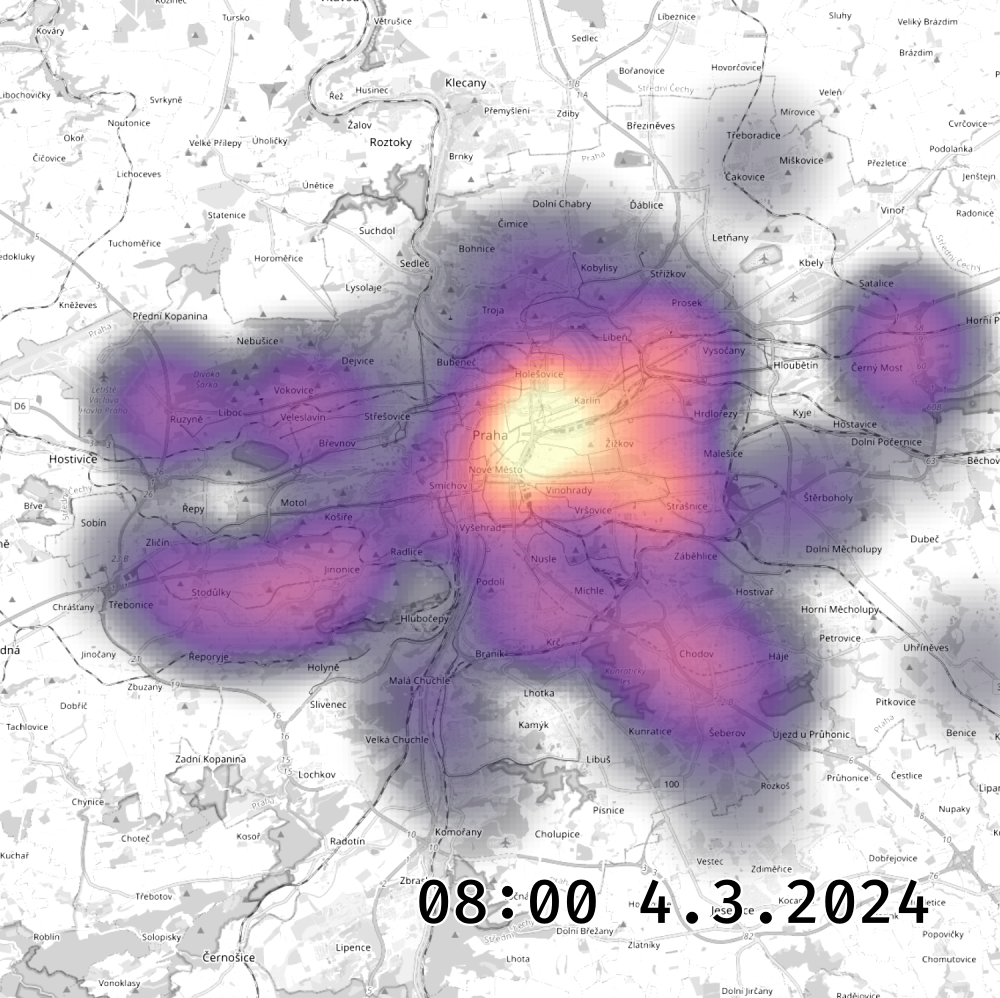
\includegraphics[width=0.45\marginparwidth]{data/timelapse/timelapse0004.png} &
        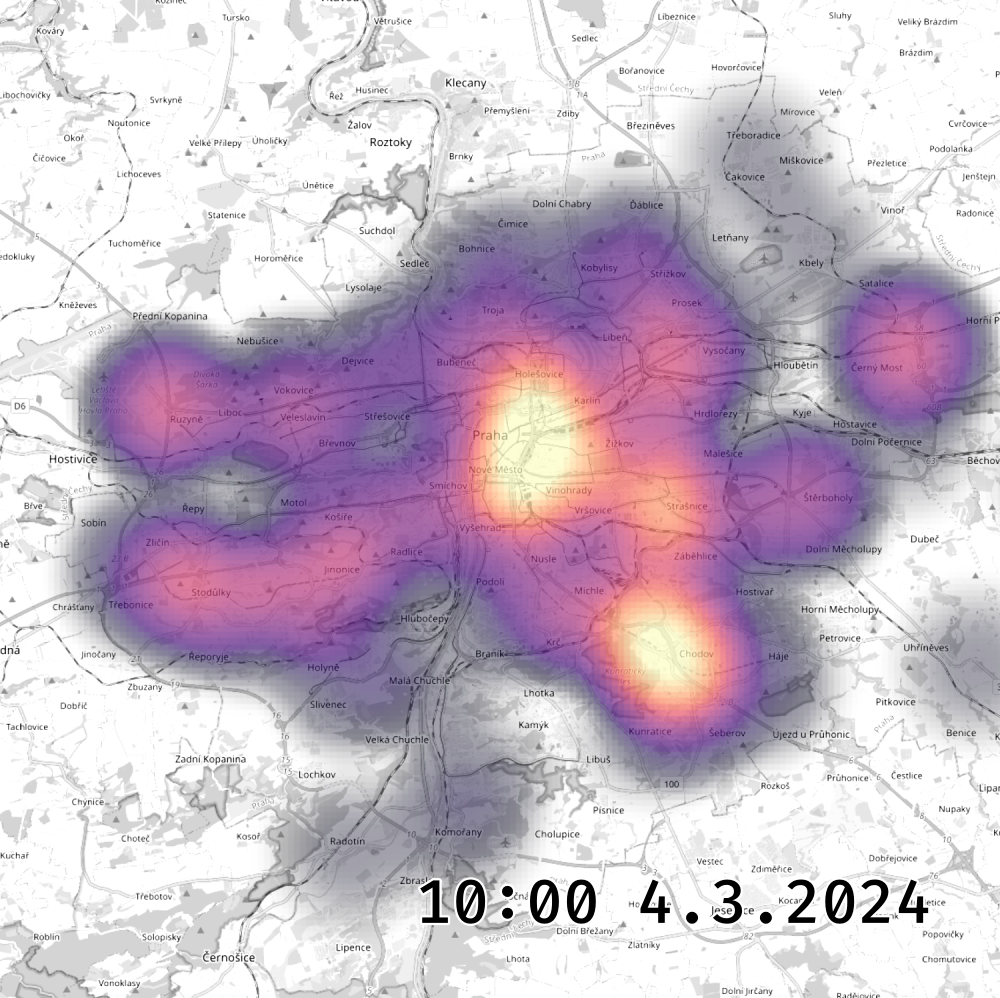
\includegraphics[width=0.45\marginparwidth]{data/timelapse/timelapse0005.png}   \\
        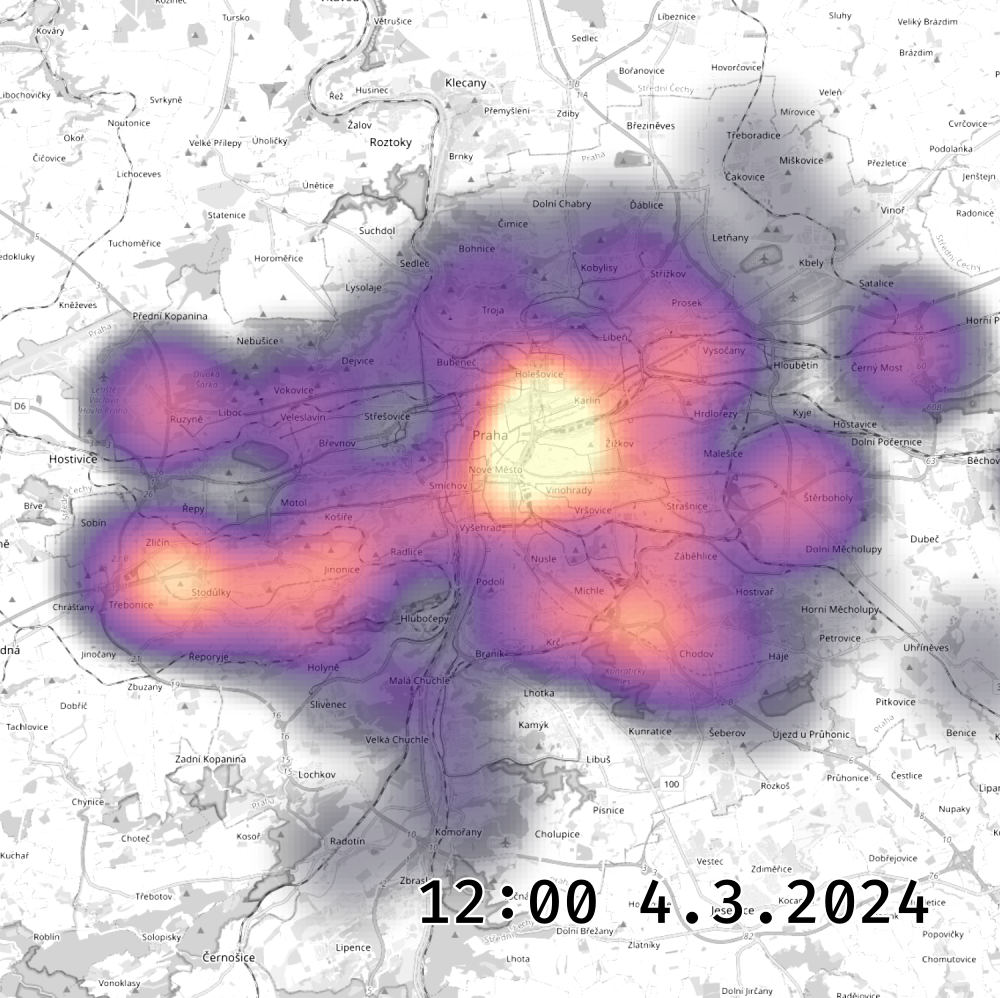
\includegraphics[width=0.45\marginparwidth]{data/timelapse/timelapse0006.png} &
        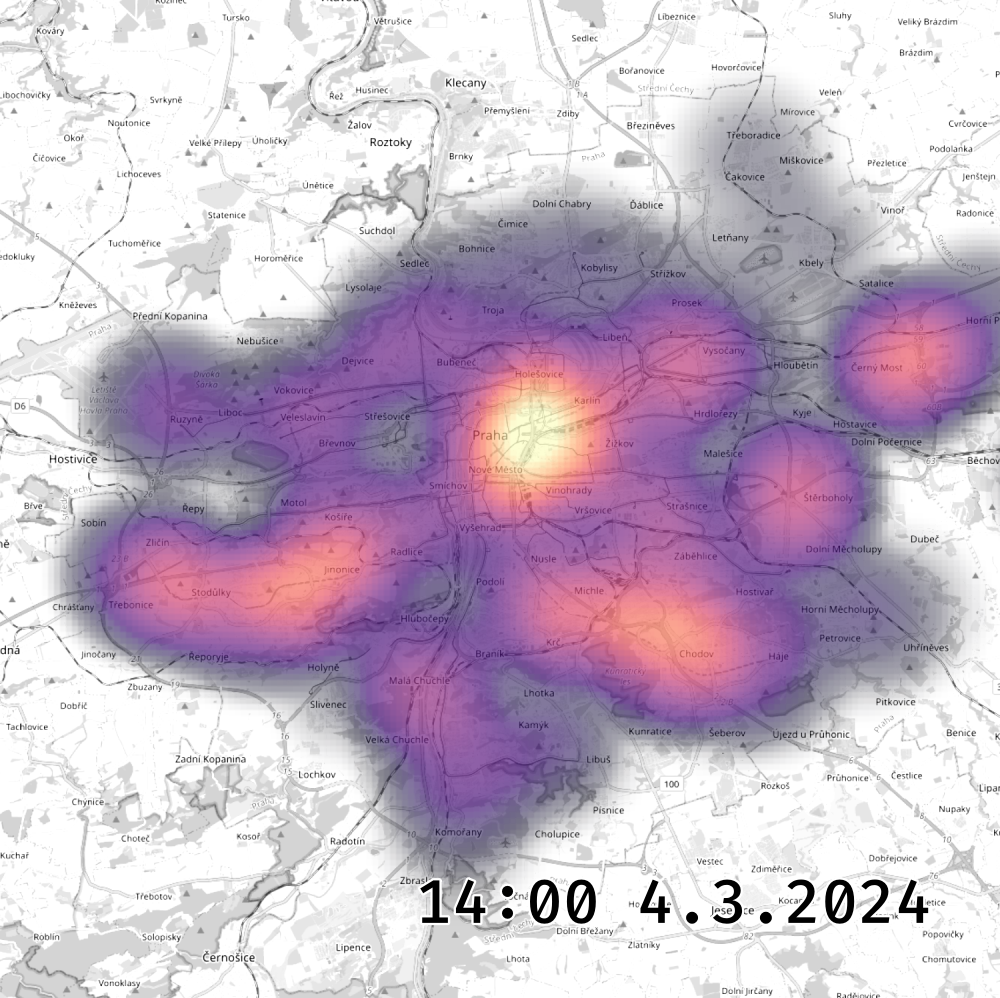
\includegraphics[width=0.45\marginparwidth]{data/timelapse/timelapse0007.png}   \\
        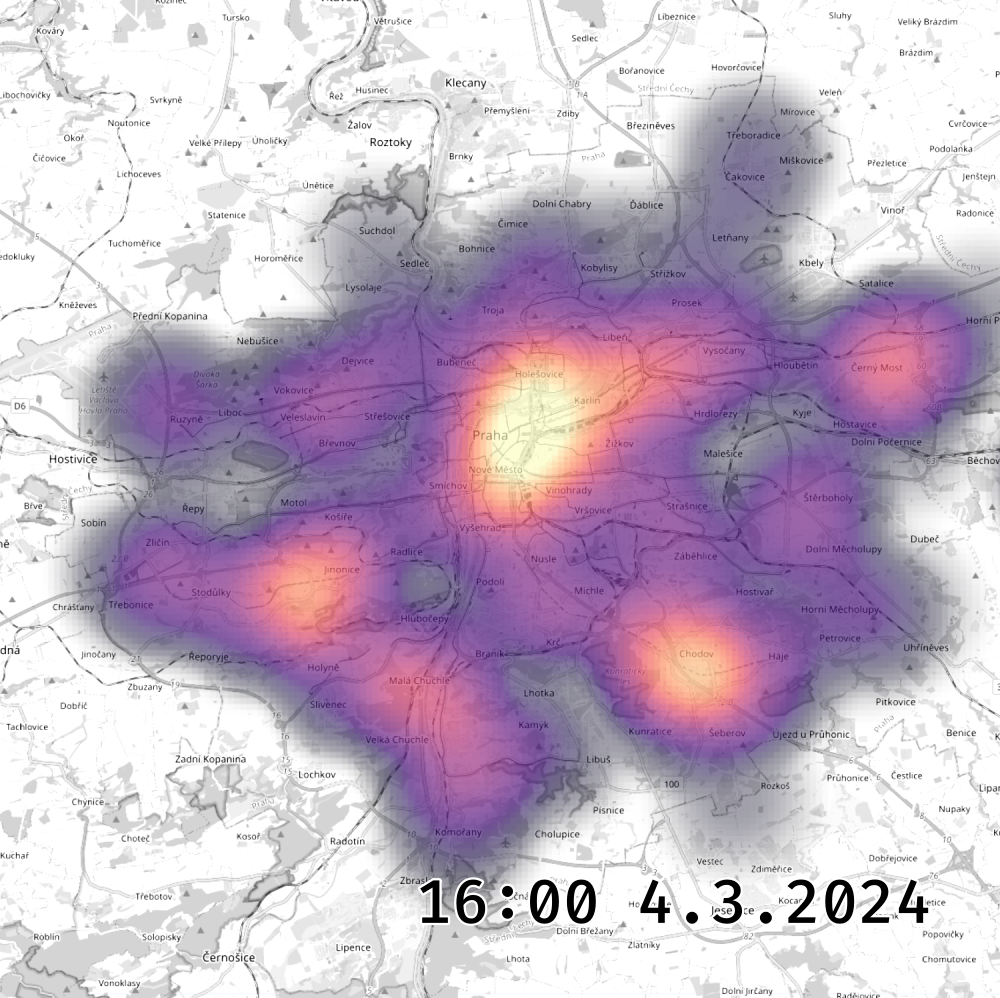
\includegraphics[width=0.45\marginparwidth]{data/timelapse/timelapse0008.png} &
        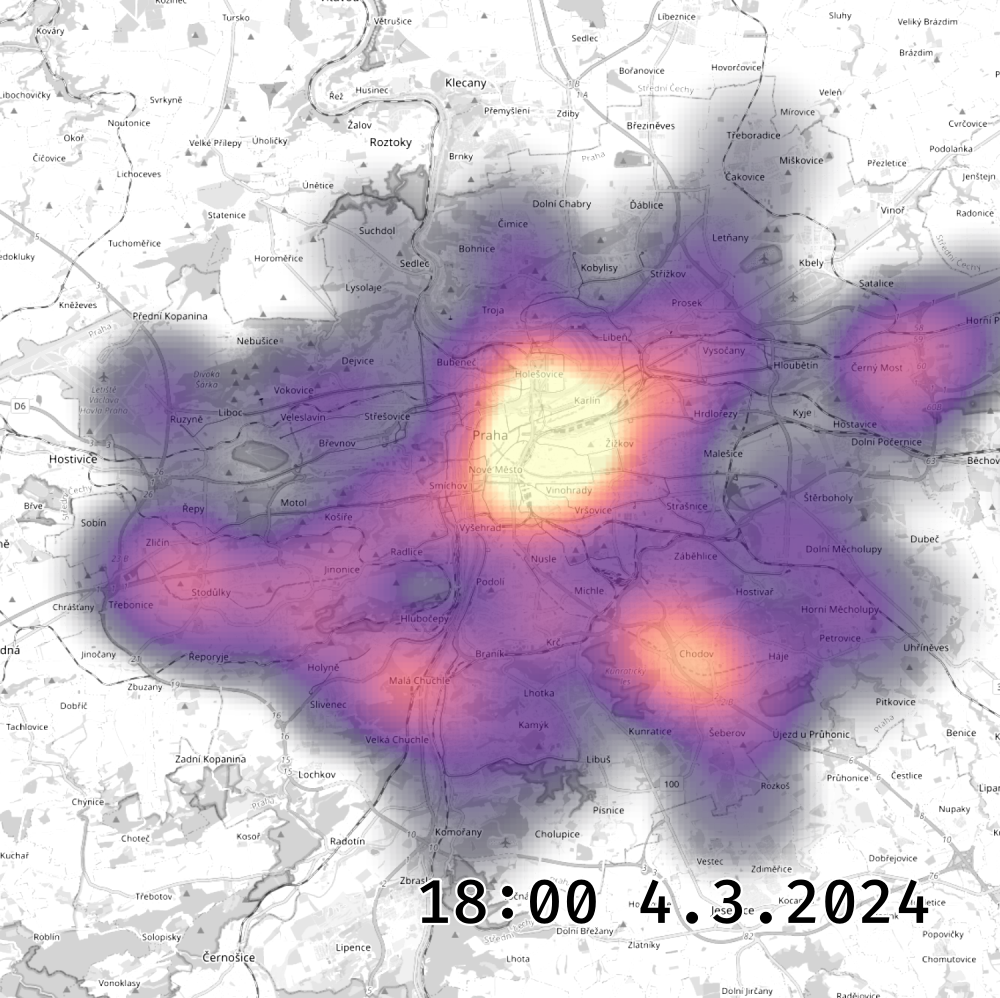
\includegraphics[width=0.45\marginparwidth]{data/timelapse/timelapse0009.png}   \\
        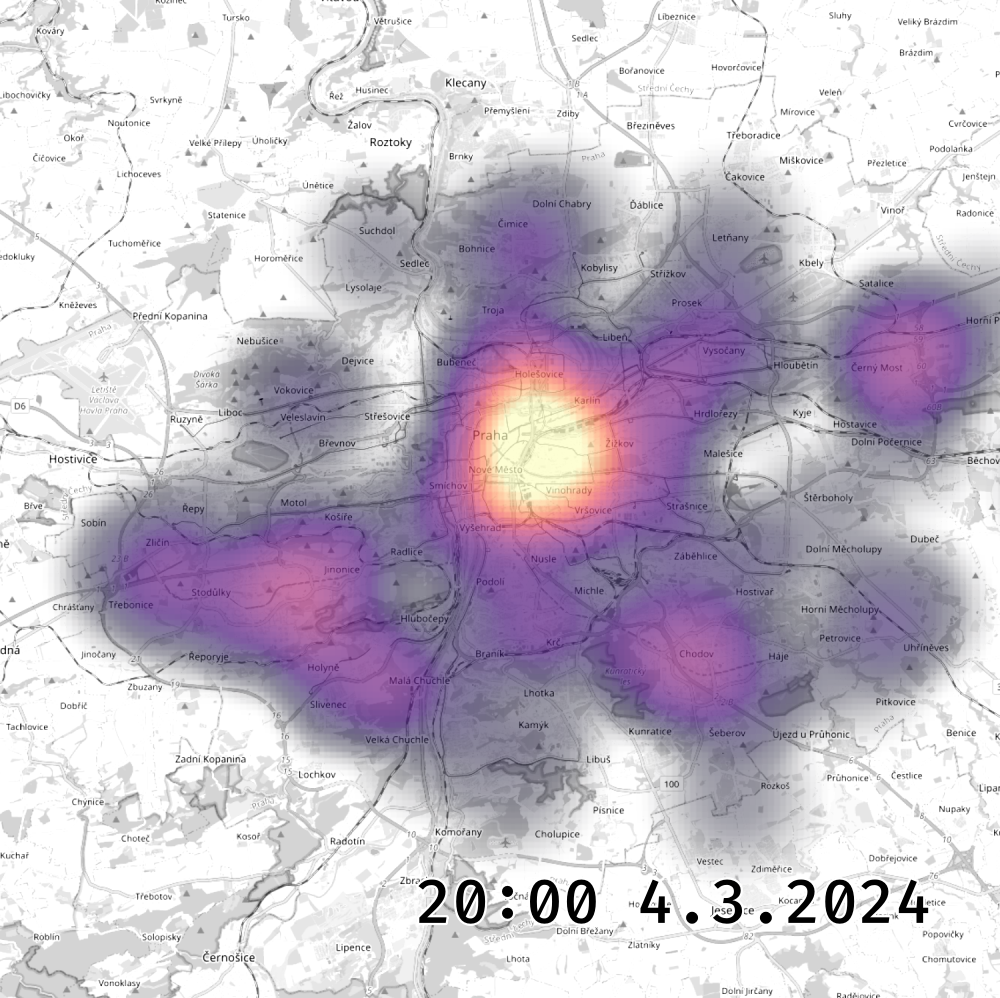
\includegraphics[width=0.45\marginparwidth]{data/timelapse/timelapse0010.png} &
        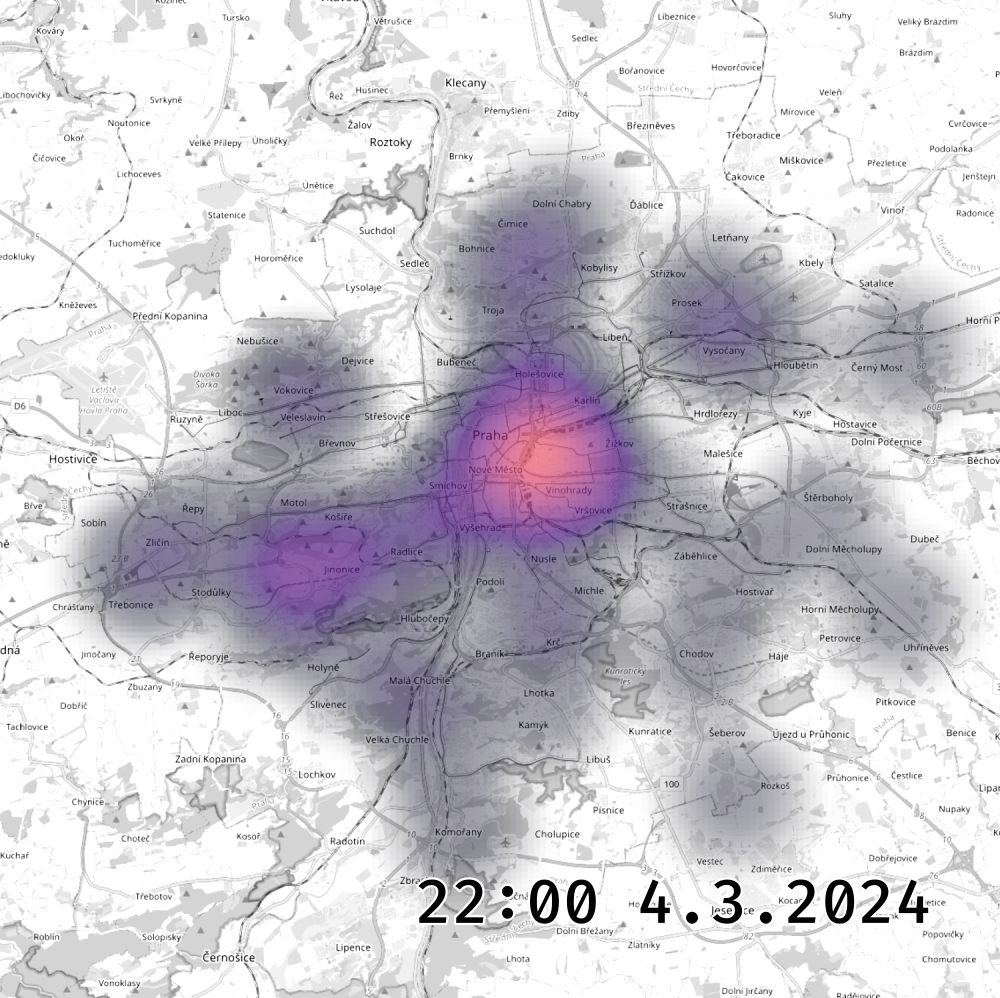
\includegraphics[width=0.45\marginparwidth]{data/timelapse/timelapse0011.png}   \\
    \end{tabular}
    \caption{Heatmap images of current charging sessions for 4th of March (Monday) separated into 12 blocks starting at 0:00. Brightest yellow denotes 15 charging sessions happenig at the given time block.}
    \label{fig:timelapse-grid-full}
\end{marginfigure}




\subsection{Transformations}

We are interested in obtaining a power demand of the charger in time. With hourly granularity. So that we can query any \acrlong{CP} at \acrlong{CS}.
We obtain \acrlong{HPC} $h^{s,c}_t$, where $s$ specifies \acrlong{CS}, $c$ \acrlong{CP} at the station. And $t$ is the hour. Where the allowed range of $t$ is limited by the start of the first session until end time of the last session.

To obtain $h^{s,c}_t$ from the sessions the following transformation takes place. For some $s,c$.

\begin{enumerate}
    \item Compute the total active timespan of the charger. Create empty hours list \[h^{s,c}_t = 0, \forall t\]
          \begin{figure}[H]
              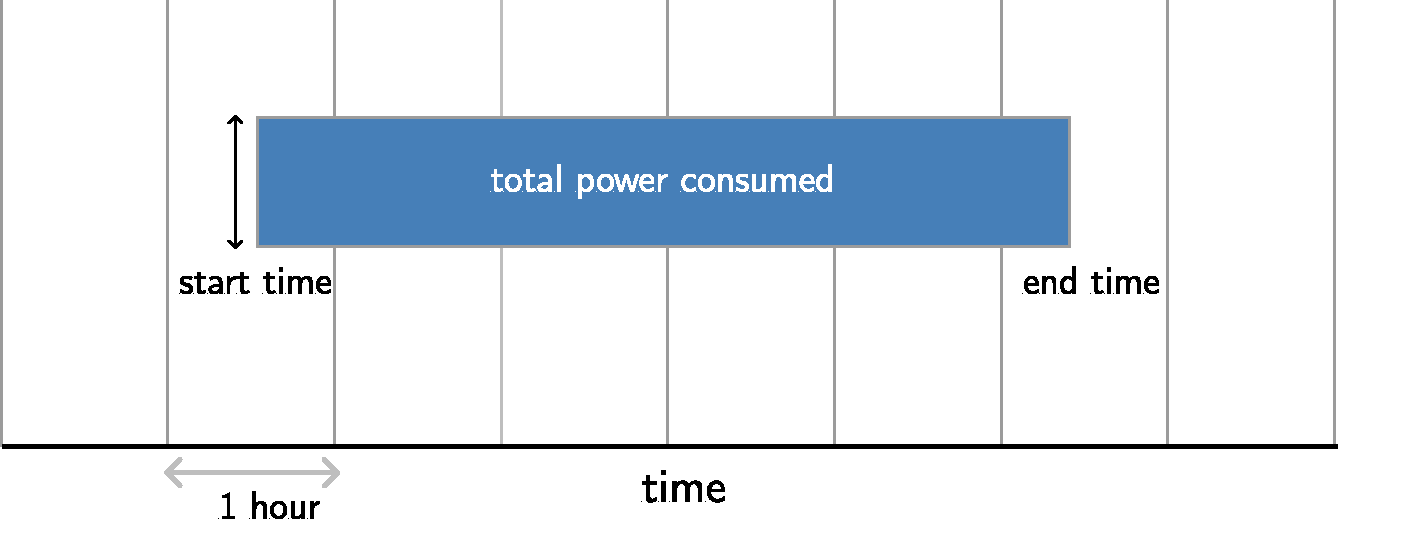
\includegraphics[width=0.8\textwidth]{data/cutting/cutting-1.pdf}
              \caption[todo]{\acrlong{CSS} overlayed with time axis.}
          \end{figure}
    \item Take each charging session $k$ $v^{c,s}_k$ for the $s,c$. And cut it into hourly chunks. And for each chunk redistribute the power consumed weighted by how big fraction of an hour the chunk occupies (this is necessary to correclty handle start and end hour chunks).
          \[
              h_t^{s,c} = \sum_{i = 1}^{|V^{s,c}|}
              \frac{
                  \mu(T \cap [t_{\text{start}}^{c,s}; t_{\text{end}}^{c,s}])
              }{
                  \mu([t_{\text{start}}^{c,s}; t_{\text{end}}^{c,s}])
              }
              *
              p_i^{c,s}, \forall t
          \]
          where $\mu$ is a function to measure length of interval. \[\mu((a;b)) \mapsto b - a\]
          \begin{figure}[H]
              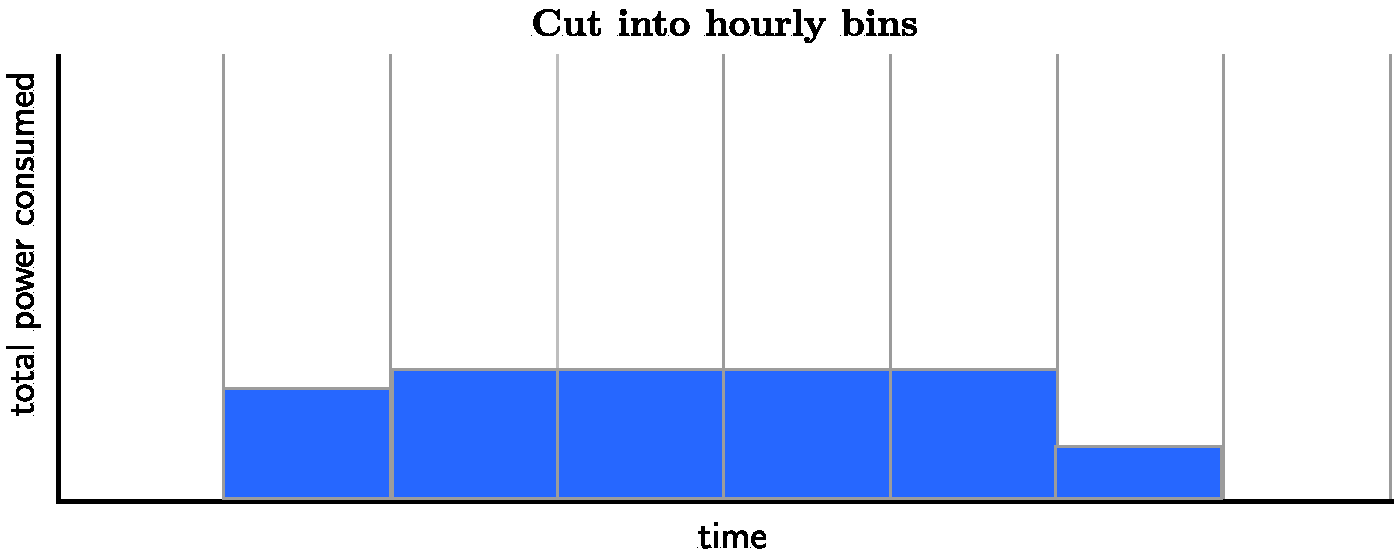
\includegraphics[width=0.8\textwidth]{data/cutting/cutting-2.pdf}
              \caption[todo]]{\acrlong{CSS} cut into hourly chunks with assigned power consumption by fraction of the hour the session occupied.}
          \end{figure}
    \item Then group the hourly power consumption into days into \acrlong{DHPC}
          \[H_d^{c,s} =
              \begin{bmatrix}
                  h^{c,s}_{d_1}    \\
                  \vdots           \\
                  h^{c,s}_{d_{24}} \\
              \end{bmatrix}
          \] where $d$ is a day and $d_i$ denotes $i$-th hour range of day $d$
\end{enumerate}


We are also interested in aggregate behaviour of the \acrlong{CP} and \acrlong{CS}. That is compute average over some day/temporal pattern. So to compute average for some $O \in \{\text{Monday}, \dots, \text{Friday} \} \times \{ \text{January}, \dots, \text{December} \}$.

Using either \acrlong{DHPC} or \acrlong{APC} an total daily power consumption ($|H^{c,s}_{d}|_1$) and normalized power consumption ($\frac{H^{c,s}_d}{|H^{c,s}_d|_1}$) are obtained.



To sumarize data derived from \acrlong{CSS}, which will be used further in this thesis:
\begin{itemize}
    \item \textbf{\acrlong{HPC}} - \lipsum[1][1-3]
    \item \textbf{\acrlong{DHPC}} - \lipsum[1][1-3]
    \item \textbf{\acrlong{APC}} - \lipsum[1][1-3]
    \item \textbf{\acrlong{TDPC}} - \lipsum[1][1-3]
    \item \textbf{\acrlong{NDPC}} - \lipsum[1][1-3]
\end{itemize}

\begin{figure}
    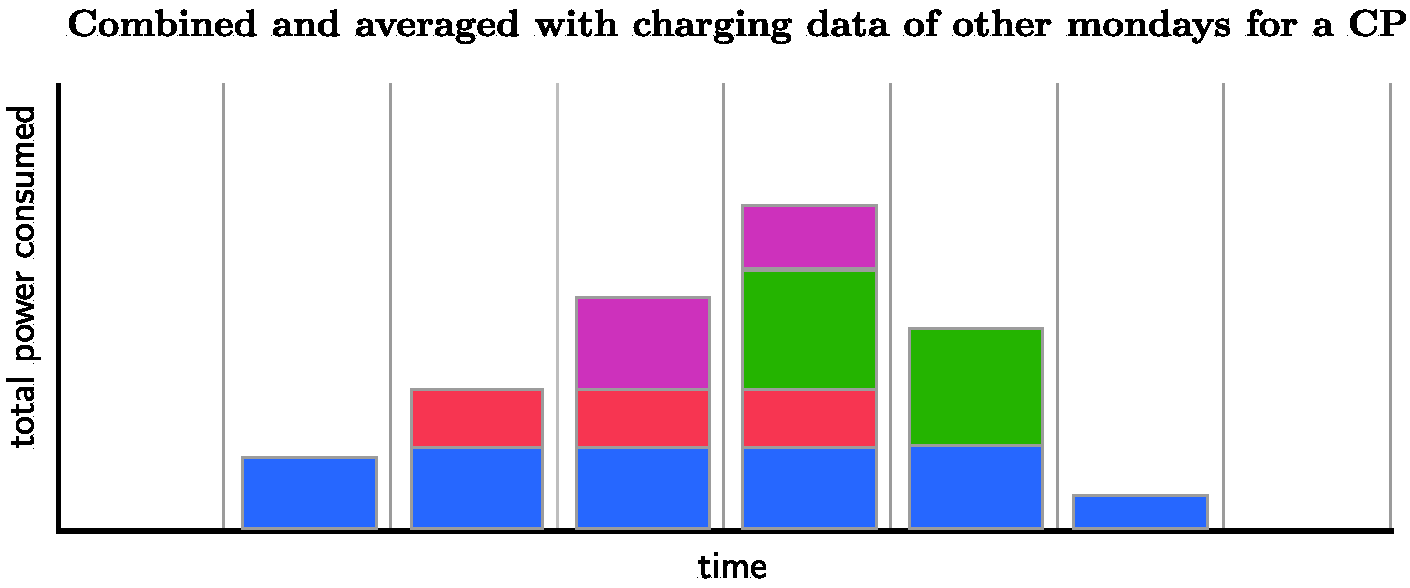
\includegraphics[width=0.8\textwidth]{data/cutting/cutting-3.pdf}
    \caption[Cutting]{\acrlong{CP} power consumption averaged over some $o \in O$ temporal pattern}
\end{figure}

\section{Basic settlement unit (ZSJ)}

\todo{todo: add motivation}

For the purposes of Czech Statistical Office Czechia is segmented into \acrfull{ZSJ}. It is a territorial element, which means a unit representing parts of the territory of a municipality with unambiguous spatial technical and urban planning conditions or catchment area groupings of residential or recreational buildings. It denotes city district, small vilages or settlements that would othervise be joined to their belonging municipality. \sidecite{ZakladniSidelniJednotka}. Their original purpose was a basic presentation unif of census data. Currently there are 23 thousand \acrshort{ZSJ} in Czechia. And of those, 953 are in Prague \sidecite{MapaZakladnichSidelnich}. The data is gathered by Czech Statistical Office from which it is was also obtained \sidecite{CeskyStatistickyUrad}.

\begin{marginfigure}
    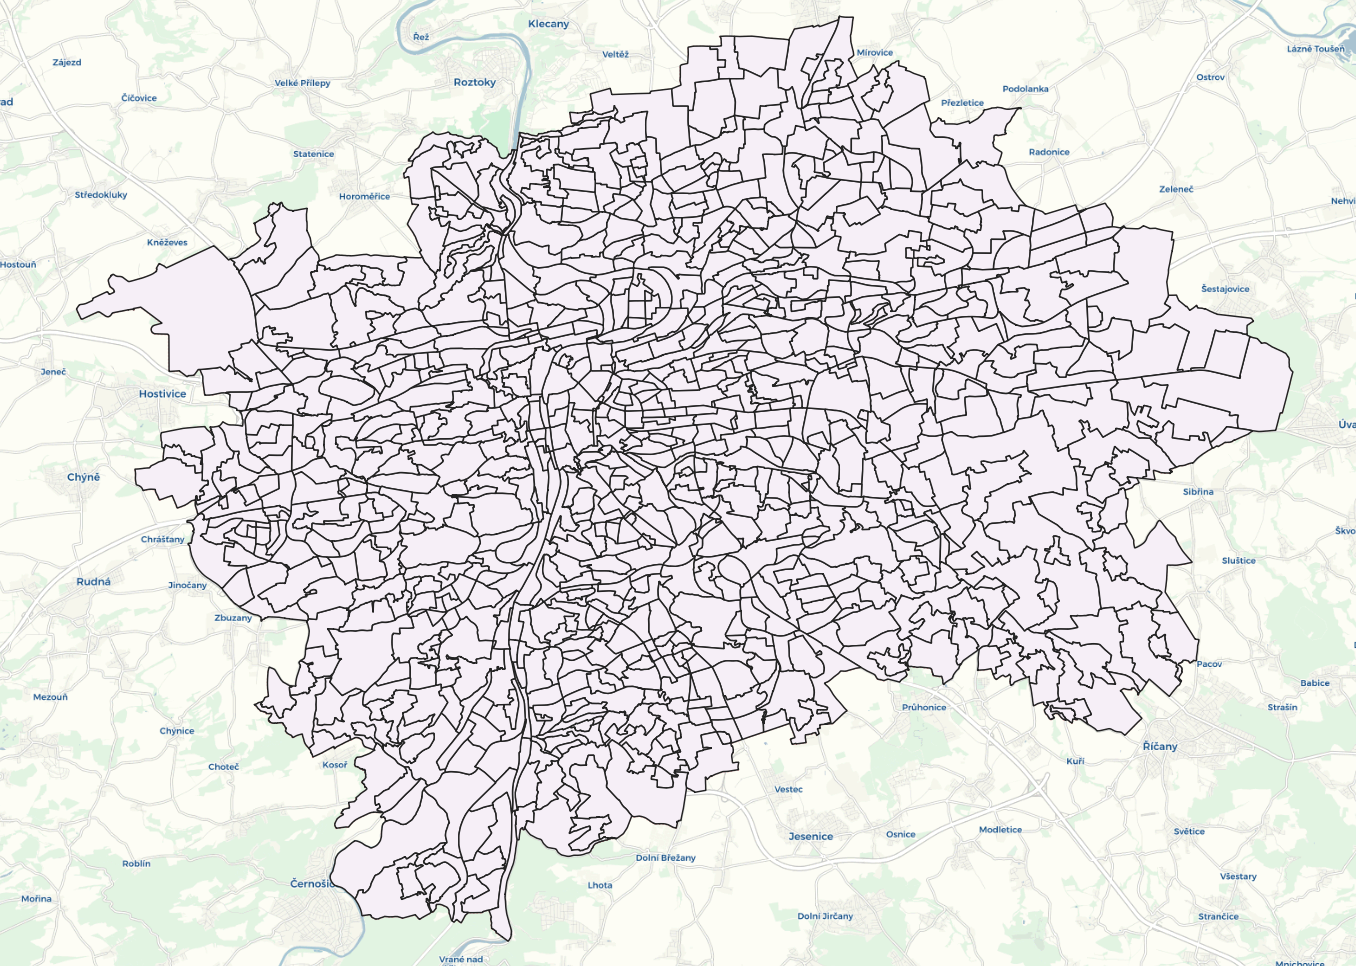
\includegraphics{data/all-zsj.png}
    \caption{}{All \acrlong{ZSJ} boundaries in Prague}
\end{marginfigure}


The dataset provides for each area
The motivated use of this dataset is that

\subsection{Description}

The dataset provides the following usefull data for each area:

\begin{itemize}
    \item \textbf{Id}: A unique identifier assigned to each ZSJ unit. This code allows for unambiguous identification of each basic settlement unit within the national registry system.
    \item \textbf{Name}: The official name (název) of the basic settlement unit, representing the commonly used designation for that specific area or settlement.
    \item \textbf{Character}: Classification indicating the functional and urban character of the ZSJ, such as residential, industrial, mixed-use, or recreational area. See visualization at \ref{fig-large:zsj-character}.
    \item \textbf{Area}: The total surface area of the ZSJ in square meters (výměra), which can be derived from geometry data but is provided as a pre-calculated attribute for convenience.
    \item \textbf{Number of addresses}: Count of valid addresses (počet adres) within the ZSJ boundaries, indicating the density of addressable locations. See visualization at \ref{fig-large:zsj-address-density}.
    \item \textbf{Population}: Number of permanent residents (počet obyvatel) recorded within the ZSJ, typically based on census data or continuous population registry. See visualization at \ref{fig-large:zsj-population-density}.
    \item \textbf{Geometry}: The spatial representation of the ZSJ boundaries as a polygon in the S-JTSK coordinate system, enabling GIS analysis and visualization of the territorial unit.
\end{itemize}

\begin{kaobox}[frametitle=Coordinate reference system - WGS84 and S-JTSK coordinate system]
    To be able to measure locations on earth as coordinates. An mathemtaical model of the earth is necessary. The most well known is WGS84(EPSG:4326)\sidecite{gmbhhttps://www.klokantech.com/WGS84WGS84} which is used by Global Positioning System (GPS). This model assumes the earth is an ellipsoid and then uses ellipsoid coordinates to be able to locate any point on the ellipsoid and thus any point on earth. This ensures it can be used worldwide. And is therefore useful for navigation. However this causes issues such as continental drift. This would render work of public offices like Czech Geodetic and Cadastral Office  more difficult due to need of recalculating the position of its objects of interest due to them shifting few centimeters each year.

    For this and historical purposes S-JTSK \sidecite{CUZKGeoportal} regional coordinate system is still employed in many public Czech offices. This system can be used only in region of Czechia and Slovakia. Is anchored to local mouments therefore mitigating issue of continental drift. And it is also a local euclidean approximation. Allowing to calculate distance between points, with some loss of precision, using ordinary euclidean distance.
\end{kaobox}

\subsection{Transformations}

The transformation performed on the data is to obtain the density instead of the absolute count. That is dividing the quantitive field values of each ZSJ with the area of its geometry polygon.

\section{People Mobility}

Poeple mobility collected from data by phone operators. Via estimation of people position by what tower the phone is connected to.

Sourced from IPR.

The data provides absolute counts of peoples commutes. To preserve privacy. As a persons origin is a place where the person(the persons phone) has spent the night and morning and the destination where the person has spent the day. Capturing data where people live and where do they go for work or to school.

\subsection{Description}

The data is provided an origin destination matrix. Where rows of the matrix are areas from where people commute and  columns are destination areas to which people commuted.

The spatial resolution is of municipalities. The data provided is provided as an average for workdays of December 2019 and March 2022. The data needed to be linked to the actual regions.



\section{Open street map}

\acrfull{POI} is a point on a map with some relevance to the domain of study. Those can be houses, shops, parking spots or landmarks.

As already mentiond \sidecite{hechtGlobalElectricVehicle2024}\sidecite{dongElectricVehicleCharging2019} have identified statistically significant releationship with \acrshort{POI} with use of linear regression . Especially \cite{hechtGlobalElectricVehicle2024} has extracted them from \acrfull{OSM}.

\acrlong{OSM}\sidecite{OpenStreetMap} is crowdsourced project aimed at constructing, maintainging and openly providing map data. The data are provided in map applications for end users for purposes like navigation. Or the data can be exported for computational analytics.

\subsection{Description}

OpenStreetMap data represents geographic features through a tagging system. The fundamental data model consists of three element types: nodes, ways, and relations. Each element can contain any number of tags in the form of key-value pairs.

For this research, we extract specific POI types relevant to charging behavior. The OSM data structure allows for detailed categorization through its tagging schema. Common tags include:

\begin{itemize}
    \item \textbf{amenity}: Services and facilities (restaurants, parking, fuel stations)
    \item \textbf{shop}: Retail establishments (supermarket, mall, convenience)
    \item \textbf{leisure}: Recreational facilities (park, sports centre, fitness centre)
    \item \textbf{tourism}: Tourist attractions (hotel, museum, attraction)
    \item \textbf{building}: Building types (residential, commercial, industrial)
    \item \textbf{landuse}: Land usage patterns (retail, residential, industrial)
    \item \textbf{road}: Highways, walkways, bikelanes, ...
\end{itemize}

\subsection{Transformations - Buildings}
\subsection{Transformations- Amenities}

To extract more points of interest. A software library \sidecite{peetzMorbZOsmPoisPbf2025} capable of extracting data from \acrshort{OSM} data was used. The extracted feautures are from \sidenote{\url{https\://wiki.openstreetmap.org/wiki/Map_feature}}. Ranging from public amenities, public transporation, accomodations, shops or tourist spots.

\begin{marginfigure}
    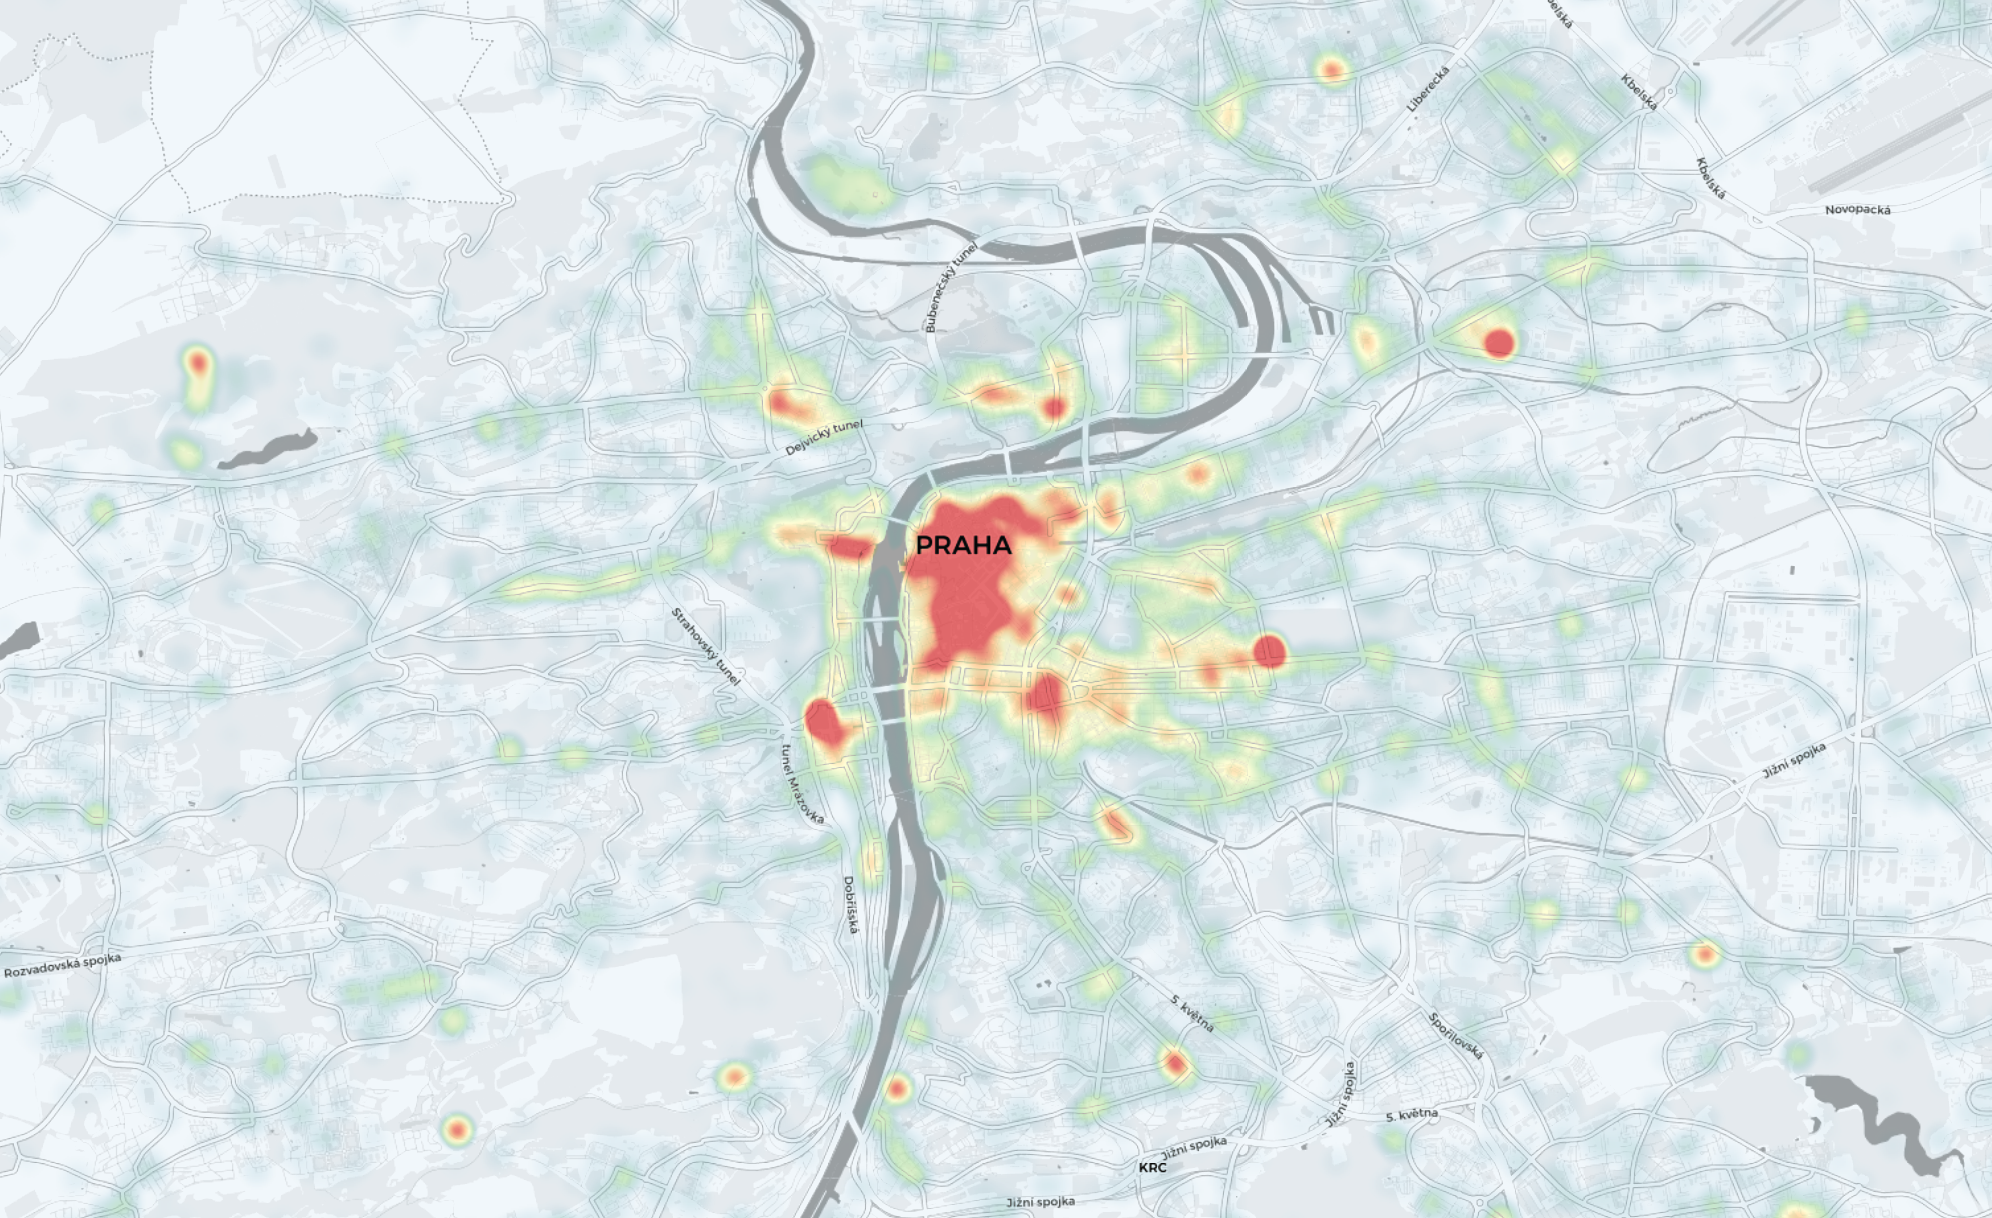
\includegraphics{data/poi-heatmap.png}
    \caption{}{PoI's in Prague heatmap}
\end{marginfigure}

% \section{Mobility Survey "Czechia in Movement (Česko v Pohybu)"}

% \subsection{Description}
% \subsection{Transformations}


\section{Spatial data transformations/feature engineering}
\label{sec:spatial-transformations}

\begin{kaobox}[frametitle=Spatial data types]

    \begin{itemize}
        \item{point} -
        \item{line/multiline} - set of connected points
        \item{polygon/multiplogyon} - representing area
    \end{itemize}
\end{kaobox}

In this section, ways how data is linked to \acrlong{CP} is mentioned. Their use is mentioned in \ref{ch:problem} for feature engineering.

\begin{itemize}
    \item[] \textbf{point in polygon} - Given a point and set of mutually disjoint areas with features. Assign features of such a area to the point according to the area the point is lying in. This method may hovewer be unreliable when the point is near a boundary with other polygons/areas. A more precise solution is spatial interpolation \sidenote{\url{https://r-spatial.org/book/12-Interpolation.html}}.
    \item[] \textbf{nearest neighbours by radius} - Given a point $\mathcal{k}$ and a set of points $\mathcal{P}$. Return subset of $\mathcal{P}$  whoose distance from $\mathcal{P}$ is less thank $K$. Also stores the distance of the point to $\mathcal{k}$. The actual distance function depends on coordinate system used.
          \[ \text{Distance}  \]
          \[\text{Distance}: \mathcal{P} \times \mathcal{P} \rightarrow \mathbb{R}^+  \]

          The $\mathcal{k}$ was set to $2000$ meters \sidecite{hechtGlobalElectricVehicle2024}. Choice of distance function depends on the coordinate system of the points.
    \item[] \textbf{nearest neighbours with importance}\sidecite{hechtGlobalElectricVehicle2024} - Similar to nearest neighbours by radius. But instead of distance it computes importance factor, computed in the following way.
          \[
              \textit{Importance}_K(a,b) = \frac{max( K - \textit{Distance}(a,b) ,0)}{K}
          \]


    \item[] \textbf{Normalization by area} - Since polygons can have varying areas and some features in absolute numbers. So normalizing the feature by the area of its polygon we obtain the density per some metric unit (usually $km^2$). For polygon $a \in A = \{a_1, \dots , a_m\}$. And funciton that assigns some feature $F \subseteq \mathbb{R}$  to polygon: $\textit{feature}, \textit{feature}: A \rightarrow F$. The density is computed like so
          \[ \text{Density}(a,f) = \frac{\textit{feature(a)}}{\textit{Area}(a)} \]
          \[\]

\end{itemize}
